\documentclass[11pt]{article}

% =========================================================================
% document style changes
% =========================================================================

\usepackage{amsmath}                    % AMS math packages
\usepackage{amssymb}                    %
\usepackage[]{graphpap}
\usepackage[T1]{fontenc}                % for \mathrm{}
\usepackage{courier}                    % for \texttt{}
\usepackage{bbm}                        % for \mathbbm{1} (indicator function)
\usepackage{booktabs}
\usepackage{graphicx}
\usepackage[font={small}]{caption}
\usepackage{subcaption}

%\setlength{\parskip}{\baselineskip}     % skip line following paragraphs
%\pagestyle{empty}                       % No page numbers
\setlength{\topmargin}{-.5in}
\setlength{\textheight}{9in}
\setlength{\oddsidemargin}{.125in}
\setlength{\textwidth}{6.25in}

\newcommand{\spc}{\vspace{0.25in}}      % Shortcut commands
\newcommand{\ds}{\displaystyle}         %\newcommand{\ds}[1]{\displaystyle{#1}}
\newcommand{\ra}{\rightarrow}
\newcommand{\Cov}{\mathrm{Cov}}
\DeclareMathOperator*{\argmax}{arg\!\max}
\DeclareMathOperator*{\argmin}{arg\!\min}

\begin{document}                        % This is where the document begins

\title{Improving Item-Item Similarity Estimation during Collaborative Filtering}
\author{Bill Chickering and Jamie Irvine\\
CS 399 with Anand Rajaraman\\
Stanford University}
\renewcommand{\today}{March 25, 2014}
\maketitle

\section*{Abstract}
\emph{Will write this when the paper is done}

\section*{Introduction}
Determining the similarity of two users or items is valuable for a number of
data-mining applications including recommender systems, product assortment and
differentiation, as well as branding. Collaborative filtering is often used to
exploit user-item rating data to make such estimates. This is typically done by
computing the Pearson correlation or cosine similarity of vector representations
of the users or items \cite{Su2009}. Given sufficient user-item rating data,
this approach can be very effective. However, when the rating data is sparse for
one or both users/items, these metrics can yield dramatic discrepancies compared
to values computed with sufficient data at a later point in time. Moreover,
these early, low-confidence measurements can be indistinguishable from later,
high-confidence measurements.  In this report, we describe two novel techniques
for estimating the true similarity of two users or items given limited common
rating data by incorporating confidence into the measurement.

To keep the present work focused, we confine ourselves to memory-based
collaborative filtering (CF) in which we work with a logical user-item matrix.
Each element of the matrix corresponds to a rating given by a particular user to
a particular item. Further, we choose to limit our analysis to item-item
similarity but note that these techniques should be equally effective at
improving user-user similarity estimation. In this representation, an item is a
vector of the ratings it has received from all users. We now formalize the
notion of item-item similarity. Two alternative models for the generation of
user-item ratings are useful in arriving at two different definitions of the
{\em true} item-item similarity.

\section*{Similarity}
\subsection*{True Item-Item Similarity}

In the first model, we imagine users are randomly presented items to rate. Given
a sufficient period of time, all users will eventually rate all items, creating
item vectors that contain provided ratings from all users. The true similarity
in this model of {\em random} rating, denoted $TrueSimRand$, is then the vector
product of two complete item vectors. That is,
\begin{align}
TrueSimRand(A, B) = \frac{\sum\limits_{u\in U}
r_{u,A}r_{u,B}}{\sqrt{\sum\limits_{u\in U} r_{u,A}^2}
\sqrt{\sum\limits_{u\in U} r_{u,B}^2}},
\end{align}
where $A$ and $B$ are items, $U$ is the set of all users and $r_{u,I}$ is the 
rating given by user $u$ to item $I$.

In the second model, we imagine an unlimited supply of users, each of whom
chooses to rate a subset of items. The lack of a rating is now meaningful since
it indicates a lack of interest of a particular user for a particular item. This
is captured by the model through a default rating of zero\footnote{We address
the issue of rating bias and the precise meaning of a zero valued ratings later
in this report.}. At any point in time, we may estimate the true similarity in
this model of {\em preferential} rating, by computing the cosine similarity of
the two item vectors. Only in the limit of inifinite time does this estimate
converge to the true similarity, which we denote $TrueSimPref$.  That is,
\begin{align}
TrueSimPref(A, B) = lim_{t\to\infty}\frac{\sum\limits_{u\in U_{AB}}
r_{u,A}r_{u,B}}{\sqrt{\sum\limits_{u\in U_A} r_{u,A}^2}
\sqrt{\sum\limits_{u\in U_B} r_{u,B}^2}},
\end{align}
where $U_A$ is the set of users who have rated $A$, $U_B$ is the set of users
who have rated $B$, and $U_{AB}$ is the set of users who have rated both $A$ and
$B$.

\subsection*{Estimating Item-Item Similarity}

Of course, most systems will never acquire ratings from all users for all items.
Nor are we able to work in the limit of infinite time. We must therefore make
estimates of the true item-item similarity using only partial information. In
the case of $TrueSimPref$, the cosine similarity computed at any point in time
serves as a simple and obvious estimate. In using this estimate, we are treating
all missing ratings as intentionally omitted. When estimating $TrueSimRand$, the
choice of how to handle missing ratings is perhaps less obvious. Following the
convention of Breese et al. \cite{Breese1998}, we choose to use the Pearson
correlation\footnote{The Pearson correlation is traditionally characterized by
subtracting an expectation value from each dimension. This is only approximately
true in our case. We discuss the how we subtract rating biases later in this
report.} for this estimate, ignoring all ratings by users who have not rated
both items. To summarize, our naive estimates are
\begin{align}
PearSim(A, B) = \frac{\sum\limits_{u\in U_{AB}}
r_{u,A}r_{u,B}}{\sqrt{\sum\limits_{u\in U_{AB}} r_{u,A}^2}
\sqrt{\sum\limits_{u\in U_{AB}} r_{u,B}^2}}
\stackrel{?}{\approx} TrueSimRand(A, B)
\end{align}

\begin{align}
CosSim(A, B) = \frac{\sum\limits_{u\in U_{AB}}
r_{u,A}r_{u,B}}{\sqrt{\sum\limits_{u\in U_A} r_{u,A}^2}
\sqrt{\sum\limits_{u\in U_B} r_{u,B}^2}}
\stackrel{?}{\approx} TrueSimPref(A, B).
\end{align}

\section*{Problem}
Both similarity estimates primarily leverage information from common users, that
is users who have rated both items. Because of this, they perform well with a
large number of common users, but give unreliable, and dramatically varying,
results when the items have few common users. In an extreme case, if only one
user has rated item $A$ and item $B$, $PearsSim(A, B) = 1$ or $-1$. Not only is
this unlikely to be an accurate assessment of the true similarity of $A$ and
$B$, it also gives the most extreme results possible, without giving any
indication that this is a low-confidence calculation.

In this paper, we present two approaches to better approximate the
true similarity given a limited number of common reviewers. Both approaches are
motivated by probabilistic models with distributions grounded in the data. The
first method leverages the observed naive similarity estimate and the number of
common users to better estimate the true similarity. The second method leverages
the observed ratings themselves for the same ends.

\subsection*{Data}
In the following section, we will describe an off-line experiment used to
evaluate our similarity estimators. But first, we provide some details about the
data used for this work. The data, originally from Amazon.com, was acquired from
the Stanford Network Analysis Project\footnote{http://snap.stanford.edu}. It
consists of ~5.6M ratings by ~1.2M users of ~600k music items (e.g. albums and
songs). Each rating is from 1 to 5 stars and is associated with a particular
user and item at a particular time.  For practical reasons, we focus our work on
two subsets of this data. The first consists of the 13,752 item pairs having at
least 40 common users (i.e. users that have provided a rating for the item). The
second consists of the 1,312 item pairs having at least 80 common reviewers. As
discussed below, we must confine ourselves to item pairs that have many common
reviewers in order to determine a good approximation of the their true
similarity.

Before any analysis of the data, we remove the biases from each rating, as in
\cite{Koren2009}:
\begin{align}
\hat{r_{ui}} = r_{ui} - \mu_r - b_u - b_i
\end{align}
where $r_{ui}$ is the raw rating user $u$ gave item $i$, $\mu_r$ is the average
rating over the entire dataset, $b_u$ is the user bias, calculated as the
average rating from user $u$ after $\mu_r$ has been subtracted from each, and
$b_i$ is the item bias, calculated as the average rating of item $i$ after
$\mu_r$ and $b_u$ have been subtracted from each. 

\subsection*{Experiment}
Ideally, we would know {\em a priori} the true similarity for a set of item
pairs. We could then generate similarity estimates and readily determine the
true error in these estimates. But both $TrueSimRand$ and $TrueSimPref$ are
theoretical constructs and not metrics we have access to in the real world.
Fortunately, we can achieve good approximations of either $TrueSim$ given
sufficient data. We therefore define $GoldPearSim = PearSim_N$ and $GoldCosSim =
CosSim_N$ where $N$ is a large enough number of common users that $GoldSim 
\approx TrueSim$.\footnote{To calculate $GoldSim$ in practice, we use $Sim$ with
all rating data, as long as the number of common users is greater than or equal
to $N$} With a measurable $GoldSim$ as our goal, we can implement 
a simple predictivity experiment.

To obtain good $GoldSim$ values, we work only with the item pairs that have at 
least either $N=40$ and $80$ common users. These choices are a compromise 
between having enough data for statistically significant results and having 
a sufficiently large $N$ that $GoldSim \approx TrueSim$. 

In order to test predicted $TrueSim$, we construct an off-line experiment to
simulate observing sparse amounts of rating data. Our experiment reenacts  
the passing of time. Starting with all ratings withheld, we apply ratings to 
items in the order they actually occured. The similarity of item pairs is then
estimated each time the number of common users $n$ is incremented. In this way,
we can quanitatively compare various estimators by calculating their mean
squared error when approximating $GoldSim$ across pairs of items. Since 
different estimators may perform better for different degrees of sparsity, 
we compute the mean squared error for $n=1,...,N$ separately.

\section*{Score-based Method}
\subsection*{Probabilistic Model}

In our first approach, we model the probability distributions of true and 
observed similarity. The goal is to use the observed similarity score directly 
to approximate the true similarity. In this way, we can consider an abstact 
$TrueSim$ which ignores the details of $TrueSimRand$ or $TrueSimPref$. 
Similarly, we consider $Sim_n$ to be a generic observed similarity score when
the two items have $n$ common reviewers. Now, let $Y$ be a random variable 
representing the $TrueSim$ of a randomly chosen pair of items. Let $X_{n}$ be a
random variable representing the $Sim_{n}$ of a pair of items when $n$ common 
users are observed.

We model $Y$ as a Normal distribution 
\begin{align}
Y \sim N(\mu_s, \sigma_{s}^2),
\end{align}
where $\mu_s$ and $\sigma_{s}^2$ are the average similarity score and the variance
of similarity scores of all pairs of items, respectively. Figure 1 shows the
distributions of $GoldSim$, which motivates a Gaussina model for $TrueSim$.

\begin{figure}[!htbp]
    \centering
    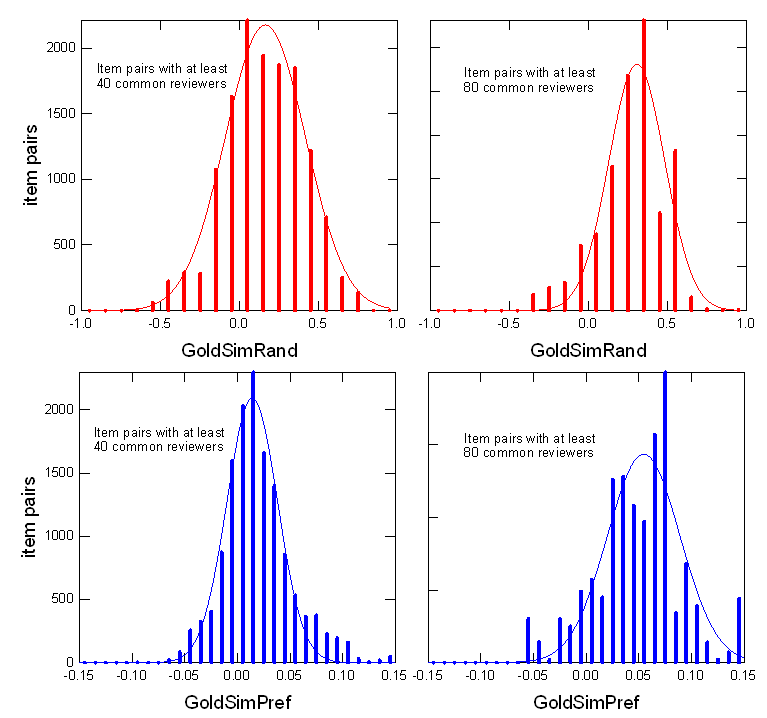
\includegraphics[width=0.8\textwidth]{Histograms.png}
	\caption{Histograms of {\em GoldPearSim} (top) and {\em GoldCosSim}
(bottom) for training datasets containing at least 40 common reviewers (left)
and 80 common reviewers (right).}
    \label{fig:Histograms}
\end{figure}


Since $X_n$ represents
a noisy reading of the true similarity $Y$, we model $X_n | Y=y$ as a Gaussian
error around $y$:
\begin{align}
(X_n | Y=y) \sim N(y, \sigma_{err, n}^2)
\end{align}
Note that $\sigma_{err, n}^2$ represents how noisy $Sim_n$ is as an estimate of
$TrueSim$ and therefore should decrease as $n$ increases. The probability
distribution of $X_n$ is illustrated in Figure 2.

\begin{figure}[!htbp]
    \centering
    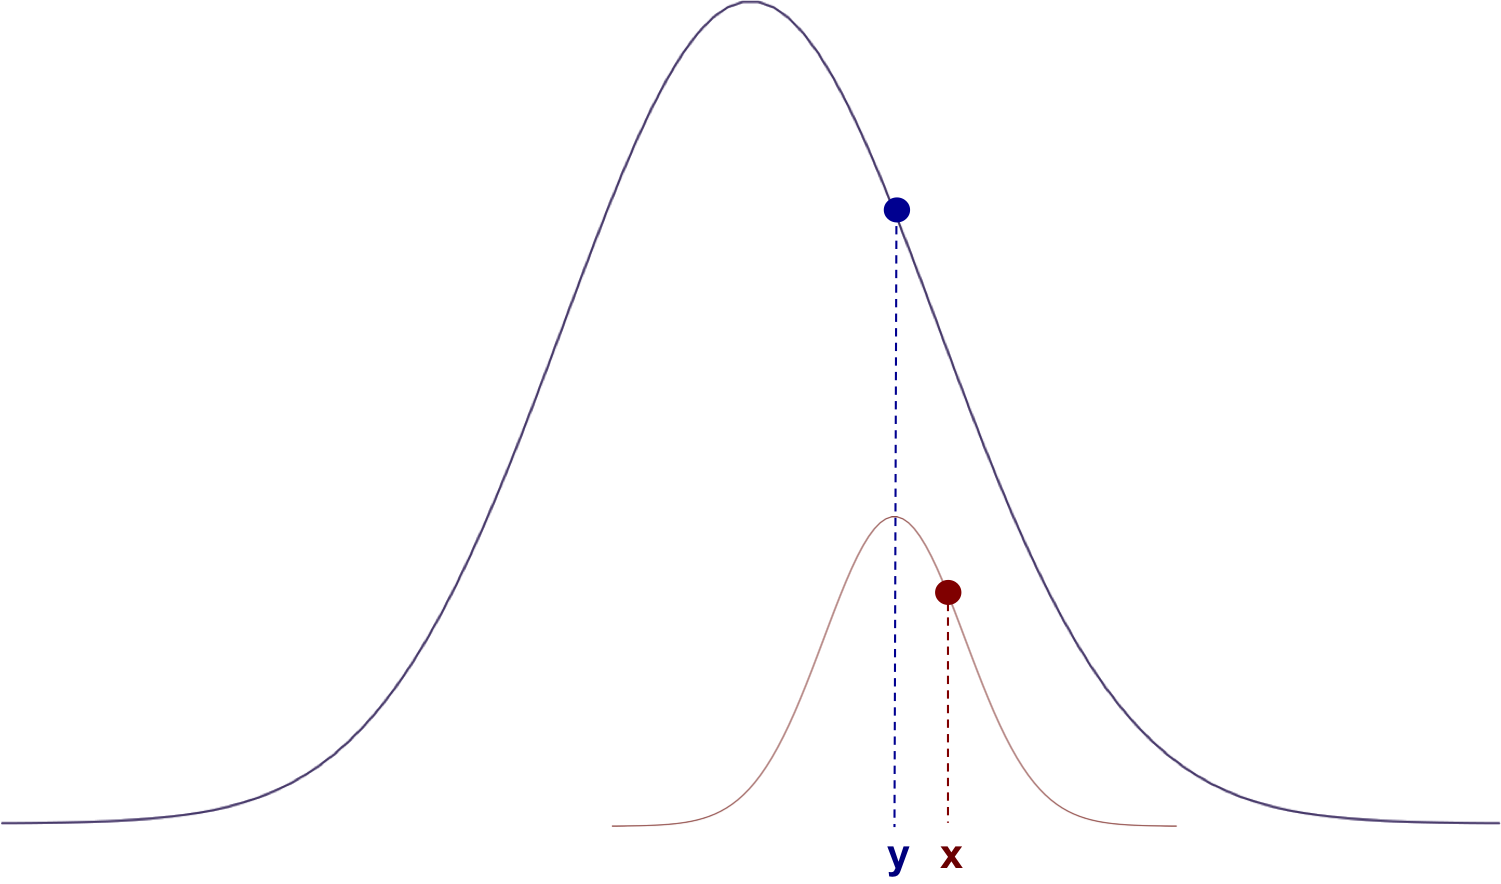
\includegraphics[width=0.7\textwidth]{twonormals.png}
	\caption{The blue curve represents $Y$, the distribution of true
    similarities between a random pair of items. The red curve represents $X|Y$,
    the observed similarity when a small number of common users exist.}
    \label{fig:two_normals}
\end{figure}

The problem of approximating $TrueSim$ given $Sim_n$ can now be seen as finding
the value of $Y$ that most likely produced $X_n$. In other words we desire the
Maximum Likelihood Estimate of $Y | X_n$:
\begin{align}
\hat{y} &= \argmax_yP(Y=y|X_n=x) 
\\&= \argmax_y\left[\frac{P(X_n=x | Y=y)P(Y=y)}{P(X_n=x)}\right]
\\&= \argmax_y\left[P(X_n=x|Y=y)P(Y=y)\right]
\\&= 
\argmax_y\left[\frac{1}{\sigma_{err,n}\sqrt{2\pi}}\exp{\left(\frac{-(x-y)^2}
{2\sigma_{err,n}^2}\right)}
\frac{1}{\sigma_{s}\sqrt{2\pi}}\exp{\left(\frac{-(y-\mu_s)^2}
{2\sigma_{s}^2}\right)}\right]
\\&= \argmin_y\left[\frac{(x-y)^2}{2\sigma_{err,n}^2} +
\frac{(y-\mu_s)^2}{2\sigma_{s}^2}\right]
\\&= \argmin_y\left[\left(\sigma_{s}^2+\sigma_{err,n}^2\right)y^2 - 
2\left(\sigma_{s}^2x+\sigma_{err,n}^2\mu_s\right)y\right]
\end{align}
We find the exact minimum by taking the derivative with respect to $y$ and
setting it to zero:
\begin{align}
\frac{d}{dy}\left[\left(\sigma_{s}^2+\sigma_{err,n}^2\right)y^2 - 
2\left(\sigma_{s}^2x+\sigma_{err,n}^2\mu_s\right)y\right]
&= 2\left(\sigma_{s}^2+\sigma_{err,n}^2\right)y - 
2\left(\sigma_{s}^2x+\sigma_{err,n}^2\mu_s\right) 
\\&= 0
\end{align}
This produces the following linear equation for $\hat{y}$ in terms of $x$
\begin{align}
\hat{y} &=
\frac{\sigma_{s}^2x+\sigma_{err,n}^2\mu_s}{\sigma_{s}^2+\sigma_{err,n}^2},
\end{align}
which can be rewritten as
\begin{align}
\left(\hat{y} - \mu_s\right) &= \frac{\sigma_{s}^2}{\sigma_{s}^2+\sigma_{err,n}^2}
\left(x-\mu_s\right).
\end{align}

The model suggests that there is a linear correlation between $X_n$ ($Sim_n$)
and $Y$ ($TrueSim$).\footnote{It is worth noting that despite the resemblance to
Slope One Predictors \cite{Lemire1998}, this is a fundamentally different
technique. Here, we have a linear relationship between observed scores and true
scores, whereas the Slope One model seeks a linear relationship between the
ratings a user gives to different items.} Moreover, the best predicted $TrueSim$
is a linear combination of the average true similarity and the observed
similiarity. Since $\sigma_{err,n}^2$ is nonnegative, the slope is always less
than or equal to one. This means that, on average, the observed distance from $\mu_s$
overestimates the true distance from $\mu_s$. This is reasonable, since the prior
distribution suggests that the true similarity is likely to be near $\mu_s$.

This model requires a different parameter $\sigma_{err,n}^2$ for each $n$.  To
gain more generality, we model $\sigma_{err,n}^2$ as a function of $n$ instead
of considering them independent of each other. Recall that $\sigma_{err,n}^2$ is
the noisiness of the observed $Sim_n$ about $TrueSim$.  $Sim$ converges to
$TrueSim$ as the number of users $n$ increases.  The Central Limit Theorem
therefore motivates the intuition that the variance of $Sim$ would decrease as
the square root of $n$. Thus we model $\sigma_{err,n}^2$ as
\begin{align}
\sigma_{err,n}^2 = \frac{\alpha}{\sqrt{n}},
\end{align}
yielding the single parameter model
\begin{align}
\left(Y - \mu_s\right) = \frac{\sigma_{s}^2}{\sigma_{s}^2+\frac{\alpha}{\sqrt{n}}}
\left(X_n-\mu_s\right).
\end{align}


\subsection*{Technique and Results}
With a measurable $GoldSim$ as our predictive goal, we can apply supervised 
learning techniques. First, we find pairs of items that have at least $N$ common
users and calculate their $GoldSim$. Next we withold some of the users to 
produce estimated $Sim_n$ for $n=1,...,N$. By doing this over many pairs of 
items, we produce pairs of ($Sim_n$, $TrueSim$) across different values of $n$ 
that can be used for training. Now the parameters $\mu_s$, $\sigma_{s}^2$, and 
$\sigma_{err,n}^2$ can be approximated using the method of moments over the 
training data. The values of $\sigma_{err,n}^2$ are fit to the function 
$\frac{\alpha}{\sqrt{n}}$ and the $\alpha$ that minimizes the sum of squared 
error is computed.

The graph of Fig. 3 compares the results of three linear fits, with varying
degrees of fidelity to the probabilistic model. The most faithful fit uses
$\mu_s$, $\sigma_{s}^2$ and $\alpha$ as calculated above to predict the $GoldSim$
using Eqn (18). The next fit uses the calculated values of $\sigma_{err,n}^2$
directly, following Eqn (16) for predictions. The third fit simply uses a series
of linear regressions, one for each $n$. This model only assumes that for each
$n$, $Sim_n$ and $GoldSim$ are linearly correlated. The linear regression
technique trades the generality of the model for a better fit on the training
data.  As the results show, the trade-off is worth it.

\begin{figure}[!htbp]
    \centering
    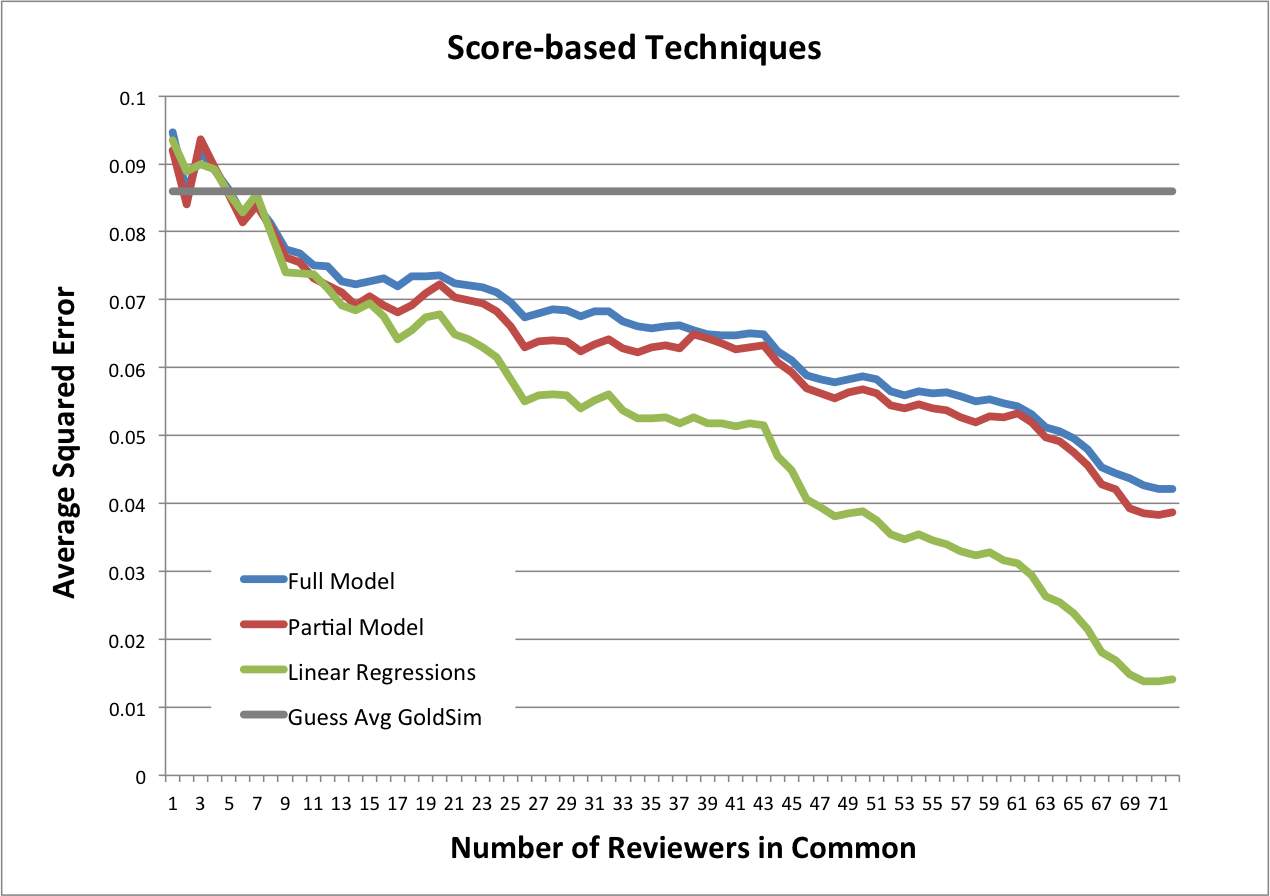
\includegraphics[width=0.7\textwidth]{LinearTechniques.png}
	\caption{Comparison of different linear techniques. For each number of
reviewers in common, $n$, the graphs represent the average squared error of
predicted $GoldSim$ calculated from the observed $Sim_n$. As a baseline, the
technique of guessing the average $GoldSim$ is included. For these experiments,
we use $Sim$ = $PearSim$ and $N=80$ for determining $GoldSim$.}
    \label{fig:Linear}
\end{figure}


\section*{Ratings-based Method}
\subsection*{Probabilistic Model}

We now construct a different probabilistic model based on the pairs of ratings
themselves. This model is readily exploited for making estimates of
$TrueSimRand$ and, to a lesser extent, $TrueSimPref$. In addition, this approach
has the added benefit of allowing us to infer implied predictions of
$TrueSimRand$ made by individual users each time they rate two items. This
latter feature allows us to define a new metric for users that we call {\em
user-predictivity}, which allows us to ascribe varying levels of confidence to
their contributions to a similarity estimate.

Let $Y$ be a random variable representing the $TrueSimRand$ of a randomly chosen
pair of items. As before, we model $Y$ as a Normal distribution
\begin{align}
Y \sim N(\mu_s, \sigma_s^2),
\end{align}
where $\mu_s$ and $\sigma_s^2$ are the average and variance of all true
similarity scores, respectively. Now, let $\vec{R} = \left(R_A~~R_B\right)$ be a
random two element vector representing the ratings given to items $A$ and $B$.
We model the conditional distribution of $\vec{R} | Y$ as a multivariate Normal
distribution
\begin{align}
(\vec{R} | Y=y) \sim N(\vec{\mu_r}, \mathbf{\Sigma_y}),
\end{align}
where $\vec{\mu_r} = (\mu_r~~\mu_r)$ are the average ratings and
$\mathbf{\Sigma_y}$ is the $y$-dependent $2\times2$ covariance matrix.  Since
$y$ is the $TrueSimRand$ score, it can be thought of as the Pearson correlation
over the distribution of ratings $R_A | Y$ and $R_B | Y$. Assuming that the
variance of individual ratings $\sigma_r^2$ is independent of $y$, we have 
\begin{align}
y = \frac{\Cov{\left[R_A | Y=y , R_B | Y=y\right]}}{\sigma_r^2},
\end{align}
It therefore follows that if the ratings are indeed normally distributed 
then the covariance matrix is related to the true similarity $y$ by
\begin{align}
\mathbf{\Sigma_y} = \sigma_r^2 \cdot
\left[ \begin{array}{cc}  1 & y \\ y & 1 \end{array} \right].
\end{align}

Using this model, we may view the problem of estimating the similarity $Y$ of
items $A$ and $B$ that most likely produced ratings $R_A$ and $R_B$ as
that of finding the Maximum Likelihood Estimate of $Y | \vec{R}$:
\begin{align}
\hat{y} &= \argmax_yP(Y=y|\vec{R}=\vec{r}) 
\\&= \argmax_y\left[\frac{P(\vec{R}=\vec{r} |
Y=y)P(Y=y)}{P(\vec{R}=\vec{r})}\right]
\\&= \argmax_y\left[P(\vec{R}=\vec{r}|Y=y)P(Y=y)\right]
\\&=
\argmax_y\left[\frac{1}{2\pi\sqrt{\left|\mathbf{\Sigma_y}\right|}}\exp{\left(-\frac{1}{2}
(\vec{r} - \vec{\mu_r})^\mathrm{T}\mathbf{\Sigma_y}^{-1}(\vec{r} - \vec{\mu_r})\right)}
\frac{1}{\sigma_{s}\sqrt{2\pi}}\exp{\left(\frac{-(y-\mu_s)^2}
{2\sigma_{s}^2}\right)}\right]
\\&= \argmin_y\left[(\vec{r} -
\vec{\mu_r})^\mathrm{T}\mathbf{\Sigma_y}^{-1}(\vec{r} - \vec{\mu_r}) + \frac{(y -
\mu_s)^2}{\sigma_{s}^2} + \ln{\left|\mathbf{\Sigma_y}\right|} \right]
\\&=
\argmin_y\left[\vec{r^\prime}^\mathrm{T}\mathbf{\Sigma_y}^{-1}\vec{r^\prime}
 + \frac{(y - \mu_s)^2}{\sigma_{s}^2} + \ln{\left|\mathbf{\Sigma_y}\right|} \right]
\\&= \argmin_y\left[\frac{1}{\sigma_r^2}\frac{1}{1 -
y^2}\left[r_A^\prime(r_A^\prime - yr_B^\prime) + r_B^\prime(r_B^\prime -
yr_A^\prime)\right] + \frac{(y - \mu_s)^2}{\sigma_{s}^2} +
\ln{\left[\sigma_r^2(1 - y^2)\right]} \right],
\end{align}
where we used the fact that
\begin{align}
\mathbf{\Sigma_y}^{-1} = \frac{1}{\sigma_r^2}
\left[ \begin{array}{cc}  1 & y \\ y & 1 \end{array} \right]^{-1} =
\frac{1}{\sigma_r^2}\frac{1}{1 - y^2}\left[ \begin{array}{cc}  1 & -y \\ -y & 1
\end{array} \right].
\end{align}
and that
\begin{align}
\left|\mathbf{\Sigma}\right| = \sigma_r^2(1 - y^2)
\end{align}
along with the substitution $\vec{r^\prime} = (r_A^\prime~~r_B^\prime) = \vec{r}
- \vec{\mu_r}$. Next, we find the minimum by taking the derivative with respect
to $y$ and setting it to zero:
\begin{align}
\frac{d}{dy}\left[ \frac{1}{\sigma_r^2}\frac{1}{1 -
y^2}\left[r_A^\prime(r_A^\prime - yr_B^\prime) + r_B^\prime(r_B^\prime -
yr_A^\prime)\right] + \frac{(y - \mu_s)^2}{\sigma_{s}^2} +
\ln{\left[\sigma_r^2(1 - y^2)\right]} \right] &= 0 \\
-r_A^\prime r_B^\prime \hat{y}^2 + ({r_A^\prime}^2 + {r_B^\prime}^2)\hat{y} - r_A^\prime
r_B^\prime + \frac{\sigma_r^2}{\sigma_s^2}(1 - \hat{y}^2)^2(\hat{y} - \mu_s) - \sigma_r^2(1
- \hat{y}^2)\hat{y} &= 0.
\end{align}
This final expression implicitly yields the MLE of $y$ as a function of the
ratings $r_A$ and $r_B$. That is, by constraining the parameters $\mu_r$,
$\sigma_r$, $\mu_s$, and $\sigma_s$ to realistic values (e.g. $\sigma_r,
\sigma_s > 0$), this expression defines a surface that can be used to
efficiently estimate $y$ given a pair of ratings\footnote{Note that this
equation neglects the constraint that $-1 \leq y \leq 1$. As a consequence, some
combinations of ratings and parameters can yield MLEs for $y$ that exceed $1$ in
magnitude. This is easily fixed, however, by applying this additional
constraint.}.

\subsection*{User Predictivity}

As already mentioned, the estimator $PearSim$ is unable to say much about the
similarity of two items when only provided ratings from a single common user. In
this case, $PearSim$ yields $\pm1$ (or the indeterminate value $0/0$ in the case
that both ratings are zero) depending on whether the ratings have the same sign
or not. The value of $\hat{y}$ provided by the above model rectifies this by
generating similarity estimates in the range $[-1, +1]$ given a single pair of
ratings. We therefore consider each user who rates a pair of items as implicitly
predicting the similarity of the items. A key discovery of the present work is
that the accuracy of users' predictions in a training set is correlated with the
accuracy in a test set. We exploit this finding by ascribing a quantity we call
{\em user predictivity} to each user defined as
\begin{align}
p_u = e^{-\epsilon_u/\lambda},
\end{align}
where $\lambda$ is a parameter to be learned and
\begin{align}
\epsilon_u = \frac{1}{\left|I_u\right|}
\sum_{A,B \in I_u}{\left|ModelSimRand(A, B) - GoldSimRand(A, B)\right|}
\end{align}
with $I_u$ the set of item pairs rated by user $u$. We are once again using
$GoldSim$ as a proxy for $TrueSim$ (See the {\bf Experiment} section) such that
$\epsilon_u$ is the average absolute error of user $u$'s similarity predictions.

\subsection*{Technique and Results}

The parameter values $\mu_s$ and $\sigma_s$ are obtained by fitting the
distribution of $GoldSimRand$ values in the training set (see Fig.
\ref{fig:Histograms}). For example, in the $N \geq 80$ dataset we have $\mu_s =
0.27$ and $\sigma_s = 0.25$. The choice of $\mu_r$ and $\sigma_r$ is less clear.
Some insight can be gained, however, by examining the prior distribution of
ratings for our datasets, which are shown in Fig. \ref{fig:RatingDist}.

\begin{figure}[!htbp]
    \centering
    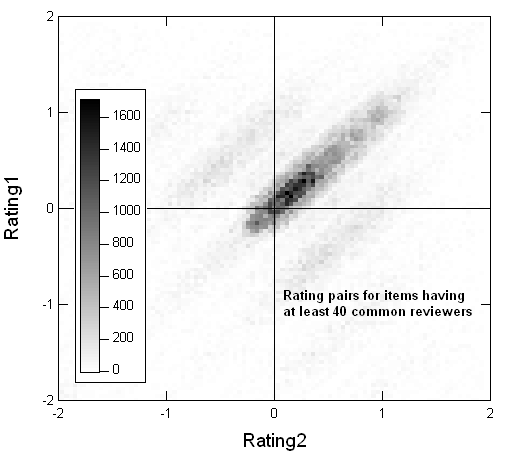
\includegraphics[width=0.7\textwidth]{RatingDist_40.png}
    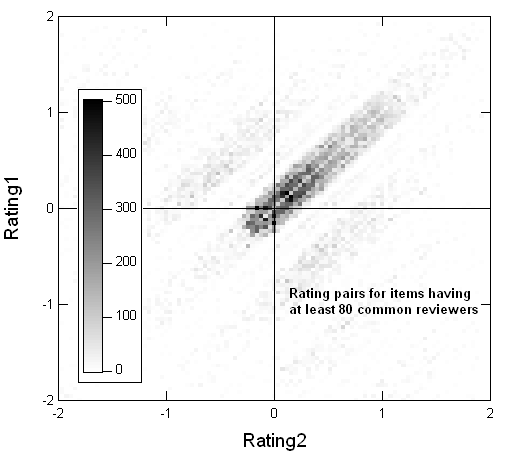
\includegraphics[width=0.7\textwidth]{RatingDist_80.png}
	\caption{Distribution of rating pairs by common reviewers for item pairs.
Top figure shows distribution for item pairs having at least 40 common
reviewers. Bottom figure shows distribution for item pairs having at least 80
common reviewers. Rating1 and Rating2 are chosen in arbitrary order.}
    \label{fig:RatingDist}
\end{figure}

Fig. \ref{fig:RetingDist} shows density plots of rating pairs, for $N \geq 40$
and $N \geq 80$. These data, together with the similarity score histograms of Fig.
\ref{fig:Histograms}, suggest that the data for our two data sets are similar
and that large biases are not introduced by varying the number of common users,
$N$. At the same time, both rating distributions reveal significant correlations
between Rating1 and Rating2 as evidenced by the elongation in the $45^\circ$
direction. This is consistent with the data of Fig. \ref{fig:Histograms}, which
shows the mean $PearSim > 0$ for both sets. Further, these data indicate a
bias toward positive values among rating pairs compared to those of ratings in
general, which have an average value of zero by construction\footnote{See
discussion of bias subtraction in {\bf Data} section.}. This latter feature
indicates that items with large numbers of common users tend to be rated higher
by their common users than by their other users since we have already subtracted
the item's average rating thereby avoiding any simple popularity effects.

We observe that while the data of Fig. \ref{fig:RatingDist} clearly do not
conform precisely to a multivariate Gaussian distribution, this approximation is
not an unreasonable one.

\begin{figure}[!htbp]
    \centering
    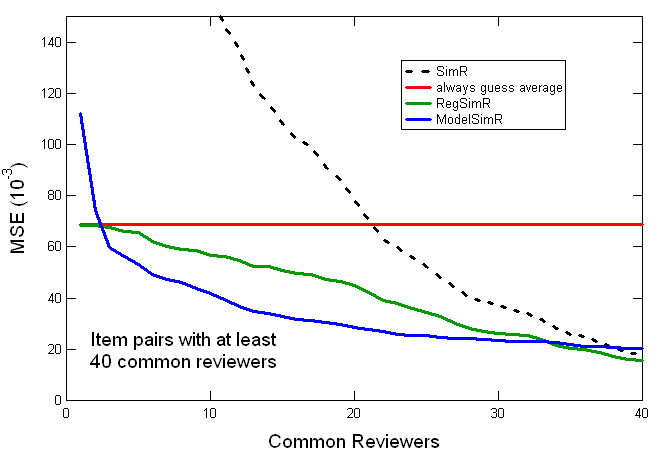
\includegraphics[width=0.9\textwidth]{MSE_SimR_40.png}
    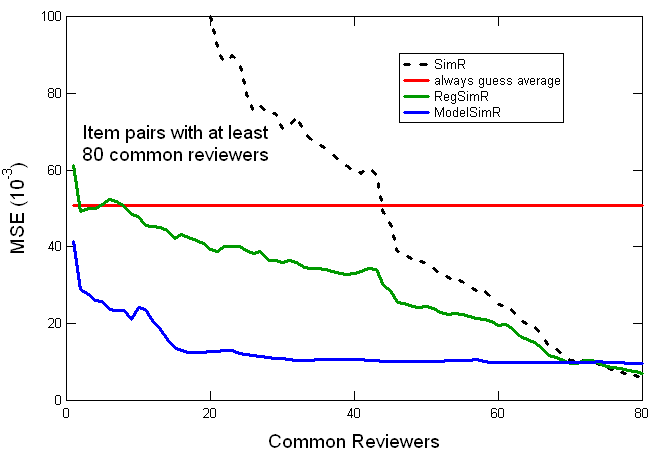
\includegraphics[width=0.9\textwidth]{MSE_SimR_80.png}
	\caption{Mean square error {\em vs} number of common reviewers, $n$, for
estimates of {\em TrueSimR} for item pairs ultimately having at least 40 common
reviewers (top) and 80 common reviewers (bottom). The dashed curve represents
{\em SimR} computed using only the ratings from the first $n$ reviewers. The
flat red line indicate the MSE that results from always guessing the average
{\em TrueSimR} from the training set. The green curve is {\em RegSimR} and the
blue curve is {\em ModelSimR}. }
    \label{fig:MSE_SimR}
\end{figure}

\begin{figure}[!htbp]
    \centering
    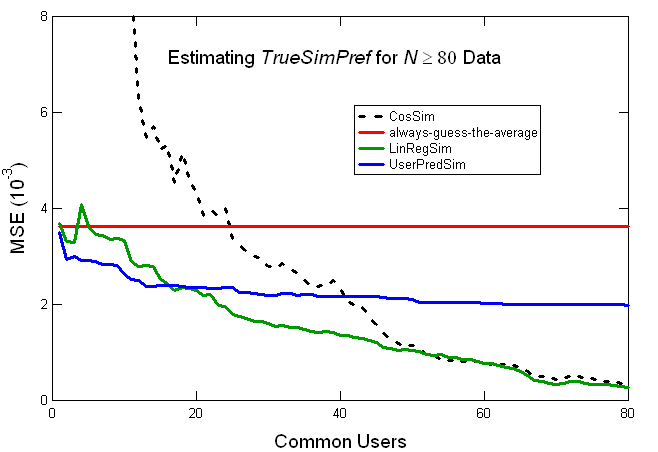
\includegraphics[width=0.9\textwidth]{MSE_SimP_80.png}
	\caption{Mean square error {\em vs} number of common reviewers, $n$, for
estimates of {\em TrueSimP} for item pairs ultimately having at least 80 common
reviewers. The dashed curve represents
{\em SimP} computed using only the ratings from the first $n$ reviewers. The
flat red line indicate the MSE that results from always guessing the average
{\em TrueSimP} from the training set. The green curve is {\em RegSimP} and the
blue curve is {\em ModelSimP}. }
    \label{fig:MSE_SimP}
\end{figure}

\section*{Conclusion}
\section*{Future Work}

\begin{thebibliography}{9}

\bibitem{Su2009}
    Xiaoyuan Su and Taghi M. Khoshgoftaar.
    ``A Survey of Collaborative Filtering Techniques.''
    \emph{Advances in Artificial Intelligence.} vol. 2009,
    Article ID 421425, 19 pages, 2009. doi:10.1155/2009/421425
\bibitem{Breese1998}
    John S. Breese, David Heckerman, and Carl Kadie, 
    ``Empirical analysis of predictive algorithms for collaborative filtering.'' 
    \emph{Proceedings of the Fourteenth conference on Uncertainty in artificial intelligence.}
    Morgan Kaufmann Publishers Inc., 1998.
\bibitem{Lemire1998}
    Daniel Lemire and Anna Maclachlan.
    ``Slope One Predictors for Online Rating-Based Collaborative Filtering.''
    \emph{SDM.} Vol. 5, 2005.
\bibitem{Koren2009}
    Yehuda Koren, Robert Bell, and Chris Volinsky. 
    ``Matrix factorization techniques for recommender systems.''
    \emph{Computer} 42.8, 2009. 30-37.

\end{thebibliography}

\end{document}
